% Created 2017-03-22 Wed 08:59
% Intended LaTeX compiler: pdflatex
\documentclass[a4paper,11pt]{article}
\usepackage[utf8]{inputenc}
\usepackage[T1]{fontenc}
\usepackage{graphicx}
\usepackage{grffile}
\usepackage{longtable}
\usepackage{wrapfig}
\usepackage{rotating}
\usepackage[normalem]{ulem}
\usepackage{amsmath}
\usepackage{textcomp}
\usepackage{amssymb}
\usepackage{capt-of}
\usepackage{hyperref}
\usepackage[margin=1in]{geometry}
\usepackage{setspace}
\onehalfspacing
\usepackage{parskip}
\usepackage{amsthm}
\usepackage{amsmath}
\usepackage{mathtools}
\usepackage{hyperref}
\usepackage{graphicx}
\usepackage{tabularx}
\usepackage{booktabs}
\usepackage{color}
\usepackage{caption}
\usepackage{subcaption}
\hypersetup{colorlinks,citecolor=black,filecolor=black,linkcolor=black,urlcolor=black}
\newtheorem{mydef}{Definition}
\newtheorem{mythm}{Theorem}
\newcommand{\dx}{\mathrm{d}}
\newcommand{\var}{\mathrm{Var}}
\newcommand{\cov}{\mathrm{Cov}}
\newcommand{\corr}{\mathrm{Corr}}
\newcommand{\pr}{\mathrm{Pr}}
\newcommand{\rarrowd}[1]{\xrightarrow{\text{ \textit #1 }}}
\renewcommand\chaptername{Lecture}
\DeclareMathOperator*{\plim}{plim}
\newcommand{\plimn}{\plim_{n \rightarrow \infty}}
\setcounter{secnumdepth}{2}
\author{Zheng Tian}
\date{}
\title{Lecture 7: Hypothesis Test and Confidence Intervals of Linear Regression with a Single Regressor}
\hypersetup{
 pdfauthor={Zheng Tian},
 pdftitle={Lecture 7: Hypothesis Test and Confidence Intervals of Linear Regression with a Single Regressor},
 pdfkeywords={},
 pdfsubject={},
 pdfcreator={Emacs 25.1.1 (Org mode 9.0.3)}, 
 pdflang={English}}
\begin{document}

\maketitle
\setcounter{tocdepth}{1}
\tableofcontents



\section{Introduction}
\label{sec:orgca67df3}

This chapter consists of two parts. The first part concerns hypothesis
testing for a single coefficient in a simple linear regression
model. The basic concepts and ideas of hypothesis testing in this
chapter can be naturally adopted in multiple regression models
(Chapters 6 and 7). The second part goes back to some estimation
issues, including a binary regressor, homoskedasticity versus
heteroskedasticity, as well as the Gauss-Markov theorem, one of the
most fundamental theories regarding the OLS estimation. Finally,
this chapter ends up with the small sample properties of the
t-statistics.

One of the features of this textbook is that it introduces the
heteroskedasticity-robust standard error of the OLS estimators, which
is considered as a general case and homoskedasticity as a special
case. This is contrary to the common layouts of an Econometrics
textbook that often first gives the assumption of homoskedasticity,
which is a component of the classical OLS assumptions (equivalent to
the three least squares assumptions plus the assumption of the
homoskedastic and conditionally normally distributed errors). Then
treat heteroskedasticity as a violation to these assumptions. Also,
you should be aware that most discussions of the sample distributions
in this textbook are in the context of a large sample, while the small
sample statistical properties are not the focus.


\section{Testing Hypotheses about One of the Regression Coefficients}
\label{sec:orgb06cc80}

\subsection{A brief review of basic concepts in hypothesis tests}
\label{sec:org81c1e0c}

Let's quickly review what we have learned in Lecture 3 about
hypothesis tests, taking an example of testing the true value of the
population mean from a random sample.

\subsubsection*{The null versus alternative hypotheses}
\label{sec:org5f5bfde}

We want to test two contrasting hypotheses, the null hypothesis versus
the alternative hypothesis. 

\begin{itemize}
\item Two-sided tests: 
$$H_0:\; E(Y) = \mu_{Y,0}$ v.s. $H_1:\; E(Y) \neq \mu_{Y,0}$$

\item One-sided test: 
$$H_0:\; E(Y) = \mu_{Y,0}$ v.s. $H_1:\; E(Y) > \mu_{Y,0}$$
\end{itemize}

\subsubsection*{Test statistics}
\label{sec:orgdc50b8a}

We need some tools for the testing, which is referred to as test
statistics.

\begin{itemize}
\item When \(\sigma_Y\) is known, we use the z-statistics
\[ z = \frac{\overline{Y} -
  \mu_{Y,0}}{\sigma_{\overline{Y}}} = \frac{\overline{Y} -
  \mu_{Y,0}}{\sigma_Y/\sqrt{n}} \xrightarrow{\text{ d }} N(0, 1)\]

\item When \(\sigma_Y\) is unknown, we use the standard error of
\(\overline{Y}\) and compute the t-statistic\footnote{In a small sample case, the exact distribution of the
t-statistics is the Student-t distribution with \(n-1\) degree of
freedom.}

\[ t = \frac{\overline{Y} - \mu_{Y,0}}{SE(\overline{Y})} =
  \frac{\overline{Y} - \mu_{Y,0}}{s_Y/\sqrt{n}} \xrightarrow{ \text{ d } } N(0, 1) \]
\end{itemize}

\subsubsection*{The rules for hypothesis testing}
\label{sec:org2561717}

We need to set up some rules for judging that under what
circumstances, the null hypothesis is rejected or fails
to be rejected. 

\begin{itemize}
\item Type I and type II errors
\label{sec:org27d15c7}

\begin{itemize}
\item \textbf{Type I error}. The null hypothesis is rejected when in fact it is
true.
\item \textbf{Type II error}. The null hypothesis is not rejected when in fact it
is false.
\end{itemize}

\item The significance level, the critical value, and the p-value
\label{sec:org545fa5b}

\begin{itemize}
\item \textbf{The significance level}. The pre-specified probability of type I
error.  \(\alpha = 0.05, 0.10, \text{ or } 0.01\)

\item \textbf{The critical value}. The value of the test statistic for which the
test rejects the null hypothesis at the given significance level.

For example. In a two-sided test, with the z statistic. The critical
value at the 5\% significance level is \(c_{\alpha}\) such that
\(\varPhi(c_{\alpha}) = 0.975\). Accordingly, we know \(c_{\alpha}
  \approx 1.96\).

\item \textbf{The p-value}. The p-value is the probability of drawing a statistic
at least as adverse to the null hypothesis as the one you actually
computed in your sample, assuming the null hypothesis is
correct. 

Equivalently, the p-value is the smallest significance
level at which the null hypothesis could be rejected, based on the
test statistic actually computed. 

Mathematically, the p-value is 
\[  \pr_{H_0}\left( \left| \frac{\overline{Y} - \mu_{Y,0}}{SE(\overline{Y})}
  \right| > \left| \frac{\overline{Y}^{act} - \mu_{Y,0}}{SE(\overline{Y})} \right| \right) =
  2\varPhi(-|t^{act}|) \text{ .} \]
\end{itemize}

\item Rejection rules
\label{sec:org030d7f6}

The following two statements are equivalent in terms of rejecting the
null hypothesis at the 5\% significance level. 

\begin{itemize}
\item We can reject the null if the test statistics falls into the
rejection region delimited by the critical values at the 5\%
significance level, that is, when \(|t^{act}| > c_{\alpha} = 1.96\),

\item We can reject the null if the p-value is less than the significance
level that is 5\% in this case.
\end{itemize}

The rejection rule can be illustrated using Figure \ref{fig:org313a2fc}.

\begin{figure}[htbp]
\centering
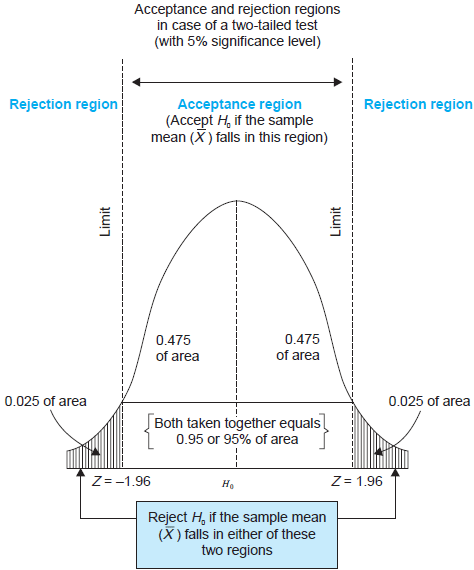
\includegraphics[width=0.7\textwidth]{./figure/fig9_1.png}
\caption{\label{fig:org313a2fc}
An illustration of a two-sided test}
\end{figure}
\end{itemize}


\subsection{Two-sided hypotheses concerning \(\beta_1\)}
\label{sec:orgc272b67}

\subsubsection*{Application to test scores}
\label{sec:org7d4ed86}

In the last lecture, we estimate a simple linear regression model for test
scores and class sizes, which yields the following estimated sample
regression function,

\begin{equation}
\label{eq:testscr-str-1e}
\widehat{TestScore} = 698.93 - 2.28 \times STR
\end{equation}

Now the question faced by the superintendent of the California
elementary school districts is whether the estimated coefficient on
\emph{STR} is valid. In the terminology of statistics, his question is
whether \(\beta_1\) is statistically significantly different from zero. 

\subsubsection*{Testing hypotheses about the slope \(\beta_1\)}
\label{sec:org3bb4787}

Note that all discussions about hypothesis testing that
follows involve only the regression with a large sample size. The
last section of this lecture touches upon the small sample properties
of the test statistics.

\begin{itemize}
\item The two-sided hypothesis
\label{sec:org3b9ba12}

\[ H_0: \beta_1 = \beta_{1,0} \text{ vs. } H_1: \beta_1 \neq \beta_{1,0} \]

The null hypothesis is that \(\beta_1\) is equal to a specific value
\(\beta_{1,0}\), and the alternative hypothesis is the opposite. 

\item The t-statistic
\label{sec:org38c85a9}

The general form of the t-statistic is

\begin{equation}
\label{eq:general-t}
t = \frac{\text{estimator} - \text{hypothesized value}}{\text{standard error of the estimator}}
\end{equation}

The t-statistics for testing \(\beta_1\) is then

\begin{equation}
\label{eq:t-stat-b1}
t = \frac{\hat{\beta}_1 - \beta_{1,0}}{SE(\hat{\beta}_1)}
\end{equation}

\item The standard error of \(\hat{\beta}_1\) is calculated as
\label{sec:org1e31c37}

\begin{equation}
\label{eq:se-b-1}
SE(\hat{\beta}_1) = \sqrt{\hat{\sigma}^2_{\hat{\beta}_1}}
\end{equation}
where
\begin{equation}
\label{eq:sigma-b-1}
\hat{\sigma}^2_{\hat{\beta}_1} = \frac{1}{n} \frac{\frac{1}{n-2} \sum_{i=1}^n (X_i - \bar{X})^2 \hat{u}^2_i}{\left[ \frac{1}{n} \sum_{i=1}^n (X_i - \bar{X})^2 \right]^2}
\end{equation}

\item How to understand Equation \ref{eq:sigma-b-1}
\label{sec:org9fac894}

\begin{itemize}
\item The population variance of \(\beta_1\) is 
\[ \sigma^2_{\hat{\beta}_1} = \frac{1}{n} \frac{\var\left( (X_i - \mu_X)u_i \right)}{\left( \var(X_i) \right)^2} \]

\item The denominator in Equation (\ref{eq:sigma-b-1}) is a consistent
estimator of \(\var(X_i)^2\).

\item The numerator in Equation (\ref{eq:sigma-b-1}) is a consistent
estimator of \(\var((X_i - \mu_X)u_i)\), adjusted by \(n-2\) degrees
of freedom.

\item The standard error computed from Equation (\ref{eq:sigma-b-1}) is
the \textbf{heteroskedasticity-robust standard error}, which will be
explained in detail shortly in this lecture.
\end{itemize}

\item Compute the p-value
\label{sec:org3068a96}

The p-value is the probability of observing a value of \(\hat{\beta}_1\)
at least as different from \(\beta_{1,0}\) as the estimate actually
computed (\(\hat{\beta}^{act}_1\)), assuming that the null hypothesis is
correct. Accordingly, under the null hypothesis, the p-value for
testing \(\beta_1\) can be expressed with a probability function as

\begin{equation*}
\begin{split}
p\text{-value} &= \pr_{H_0} \left( | \hat{\beta}_1 - \beta_{1,0} | > | \hat{\beta}^{act}_1 - \beta_{1,0} | \right) \\
&= \pr_{H_0} \left( \left| \frac{\hat{\beta}_1 - \beta_{1,0}}{SE(\hat{\beta}_1)} \right| > \left| \frac{\hat{\beta}^{act}_1 - \beta_{1,0}}{SE(\hat{\beta}_1)} \right| \right) \\
&= \pr_{H_0} \left( |t| > |t^{act}| \right)
\end{split}
\end{equation*}

With a large sample, \(p\text{-value} = \pr\left(|t| > |t^{act}|
\right) = 2 \varPhi(-|t^{act}|)\).

The null hypothesis is rejected at the 5\% significance level if the
\(p\text{-value} < 0.05\) or, equivalently, \(|t^{act}| > 1.96\). 

\item Application to test scores
\label{sec:orgb210dc3}

The OLS estimation of the linear regression model of test scores
against student-teacher ratios, together with the standard errors of
all parameters in the model, can be represented using the following
equation, 

\begin{equation*}
\widehat{TestScore} = \underset{\displaystyle (10.4)}{698.9} - \underset{\displaystyle (0.52)}{2.28} \times STR,\; R^2 = 0.051,\; SER = 1.86
\end{equation*}

The \textbf{heteroskedasticity-robust} standard errors are reported in the
parentheses, that is, \(SE(\hat{\beta}_0) = 10.4\) and
\(SE(\hat{\beta}_1) = 0.52\). 

The superintendent's question is whether \(\beta_1\) is significant for
which we can test the null hypothesis against the alternative one as
\[ H_0: \beta_1 = 0, H_1: \beta_1 \neq 0 \]

The t-statistics is
\[ t = \frac{\hat{\beta}_1}{SE(\hat{\beta}_1)} = \frac{-2.28}{0.52}
= -4.38 < -1.96 \] 

The p-value associated with \(t^{act} = -4.38\) is approximately
0.00001, which is far less than 0.05. 

Based on the t-statistics and the p-value, we can say the null
hypothesis is rejected at the 5\% significance level. In English, it
means that the student-teacher ratios do have a significant effect on
test scores. 

\begin{figure}[htbp]
\centering
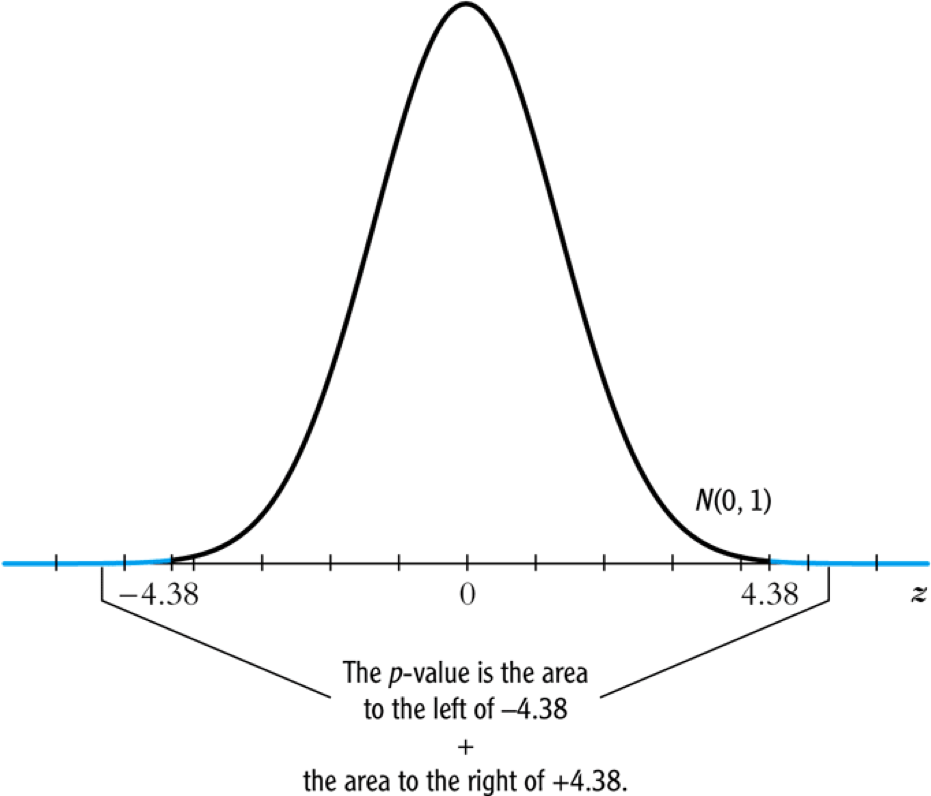
\includegraphics[width=0.7\textwidth]{figure/fig-5-1.png}
\caption{\label{fig:org8d8f514}
Calculating the p-value of a two-sided test when \(t^{act}=-4.38\)}
\end{figure}
\end{itemize}


\subsection{The one-sided alternative hypothesis}
\label{sec:orgb607691}

\subsubsection*{The one-sided hypotheses}
\label{sec:orgd33ede2}

In some cases, it is appropriate to use a one-sided hypothesis
test. For example, the superintendent of the California school
districts want to know whether class sizes have a negative effect on
test scores, that is, \(\beta_1 < 0\). 

For a one-sided test, the null hypothesis and the one-sided
alternative hypothesis are \footnote{Note that the trick here is we put the
desired hypothesis to the alternative place.}

\[ H_0: \beta_1 = \beta_{1,0} \text{ vs. } H_1: \beta_1 < \beta_{1,0} \]

\subsubsection*{The one-sided left-tail test}
\label{sec:org1c8b3b3}

\begin{itemize}
\item The t-statistic is the same as in a two-sided test
\[ t = \frac{\hat{\beta}_1 - \beta_{1,0}}{SE(\hat{\beta}_1)} \]
\item Since we test \(\beta_1 < \beta_{1,0}\), if this is true, the
t-statistics should be statistically significantly less than zero.
\item The p-value is computed as \(\pr(t < t^{act}) = \varPhi(t^{act})\).
\item The null hypothesis is rejected at the 5\% significance level when
\(\text{p-value} < 0.05\) or \(t^{act} < -1.645\).
\item In the application of test scores, the t-statistics is -4.38, which
is less than -1.645 and -2.33 (the critical value for a one-sided
test with a 1\% significance level). Thus, the null hypothesis is
rejected at the 1\% level.
\end{itemize}


\section{Confidence Intervals for a Regression Coefficient}
\label{sec:org6a72baa}

\subsection{Two equivalent definitions of confidence intervals}
\label{sec:org1b140eb}

Recall that a 95\% \textbf{confidence interval} for \(\beta_1\) has two equivalent
definitions:
\begin{enumerate}
\item It is the set of values that cannot be rejected using a two-sided
hypothesis test with a 5\% significance level.
\item It is an interval that has a 95\% probability of containing the true
value of \(\beta_1\).
\end{enumerate}

Let's go back to Figure \ref{fig:org313a2fc}. According to the first
definition, the acceptance region contains the values of the
test statistics that fail to reject the null hypothesis,
which corresponds to the values of \(\beta_1\) that cannot be rejected. 


\subsection{Construct the 95\% confidence interval for \(\beta_1\)}
\label{sec:org57bc5c6}

The 95\% confidence interval for \(\beta_1\) can be constructed using the
t-statistic, assuming that with large samples, the t-statistic is
approximately normally distributed. The 95\% critical value of a
standard normal distribution is 1.96. Therefore, we can obtain the 95\%
confidence interval for \(\beta_1\) by the following steps

\begin{gather*}
-1.96 \leq \frac{\hat{\beta}_1 - \beta_1}{SE(\hat{\beta}_1)} \leq 1.96 \\
\hat{\beta}_1 - 1.96 SE(\hat{\beta}_1) \leq \beta_1 \leq \hat{\beta}_1 + 1.96 SE(\hat{\beta}_1)
\end{gather*}

The 95\% confidence interval for \(\beta_1\) is 
\[ \left[ \hat{\beta}_1 - 1.96 SE(\hat{\beta}_1),\; \hat{\beta}_1 + 1.96
SE(\hat{\beta}_1) \right] \]


\subsection{The application to test scores}
\label{sec:org62bfc60}

In the application to test scores, given that \(\hat{\beta}_1 = -2.28\)
and \(SE(\hat{\beta}_1) = 0.52\), the 95\% confidence interval for
\(\beta_1\) is \({-2.28 \pm 1.96 \times 0.52}\), or \(-3.30 \leq \beta_1
\leq -1.26\). 

Note that the confidence interval only spans over the negative
region with zero leaving outside the interval, which implies that the
null hypothesis of \(\beta_1 = 0\) can be rejected at the 5\%
significance level.


\subsection{Confidence intervals for predicted effects of changing \(X\)}
\label{sec:org649c380}

\(\beta_1\) is the marginal effect of \(X\) on \(Y\), that is, 
\[ \beta_1 = \frac{\dx Y}{ \dx X} \Rightarrow \dx Y = \beta_1 \dx X \]
When \(X\) changes by \(\Delta X\), \(Y\) changes by \(\beta_1 \Delta X\). 

So the 95\% confidence interval for \(\beta_1 \Delta X\) is
\[ \left[ \hat{\beta}_1 \Delta X - 1.96 SE(\hat{\beta}_1) \Delta X,\;
\hat{\beta}_1 \Delta X + 1.96SE(\hat{\beta}_1) \Delta X \right] \]


\section{Regression When \(X\) is a Binary Variable}
\label{sec:orgad71cca}

\subsection{A binary variable}
\label{sec:org57c6f1f}

A \textbf{binary variable} takes on values of one if some condition is true
and zero otherwise, which is also called a \textbf{dummy variable}, a
\textbf{categorical variable}, or an \textbf{indicator variable}.

For example, 
\begin{equation*}
D_i = 
\begin{cases}
1,\; &\text{if the } i^{th} \text{ subject is female} \\
0,\; &\text{if the } i^{th} \text{ subject is male} 
\end{cases}
\end{equation*}

The linear regression model with a dummy variable as a regressor is
\begin{equation}
\label{eq:dummy-1}
Y_i = \beta_0 + \beta_1 D_i + u_i,\; i = 1, \ldots, n
\end{equation}

The coefficient on \(D_i\) is estimated by the OLS estimation method
in the same way as a continuous regressor. The difference lies in how
we interpret \(\beta_1\). 


\subsection{Interpretation of the regression coefficients}
\label{sec:orgf04ae68}

Given that the assumption \(E(u_i | D_i) = 0\) holds in Equation
(\ref{eq:dummy-1}), we have two population regression functions for
the two cases, that is,
\begin{itemize}
\item When \(D_i = 1\), \(E(Y_i|D_i = 1) = \beta_0 + \beta_1\)
\item When \(D_i = 0\), \(E(Y_i|D_i = 0) = \beta_0\)
\end{itemize}

Therefore, \(\beta_1 = E(Y_i | D_i = 1) - E(Y_i |D_i = 0)\), that is,
\textbf{the difference in the population means} between two groups represented by
\(D_i = 1\) and \(D_i = 0\), respectively.


\subsection{Hypothesis tests and confidence intervals}
\label{sec:orga4ab873}

The hypothesis tests and confidence intervals for the coefficient on a
binary variable follows the same procedure of those for a continuous
variable \(X\). 

Usually, the null and alternative hypotheses concerning a dummy variable are
\[ H_0:\, \beta_1 = 0 \text{ vs. } H_1:\, \beta_1 \neq 0 \]
Therefore, the t-statistic is 
\[ t = \frac{\hat{\beta}_1}{SE(\hat{\beta}_1)} \]
And the 95\% confidence interval is
\[ \hat{\beta}_1 \pm 1.96 SE(\hat{\beta}_1) \]


\section{Heteroskedasticity and Homoskedasticity}
\label{sec:orga06e261}

\subsection{What are heteroskedasticity and homoskedasticity?}
\label{sec:orgfdd948d}

\subsubsection*{Homoskedasticity}
\label{sec:orgb42775d}

The error term \(u_i\) is \textbf{homoskedastic} if the conditional variance of
\(u_i\) given \(X_i\) is constant for \(i = 1, \ldots, n\). Mathematically,
it says \(\var(u_i | X_i) = \sigma^2,\, \text{ for } i = 1, \ldots, n\),
i.e., the variance of \(u_i\) for all \emph{i} is a constant and does not
depend on \(X_i\).

\subsubsection*{Heteroskedasticity}
\label{sec:orgccb6b65}
In contrast, the error term \(u_i\) is \textbf{heteroskedastic} if the conditional variance of
\(u_i\) given \(X_i\) changes on \(X_i\) for \(i = 1, \ldots, n\). That is,
\(\var(u_i | X_i) = \sigma^2_i,\, \text{ for } i = 1, \ldots, n\). 

e.g.. A multiplicative form of heteroskedasticity is \(\var(u_i|X_i)
= \sigma^2 f(X_i)\) where \(f(X_i)\) is a function of \(X_i\), for
example, \(f(X_i) = X_i\) as a simplest case. 

Figure \ref{fig:homovshetero} for a visual comparison between
homoskedasticity and heteroskedasticity. 

\begin{figure}
    \centering
    \begin{subfigure}[!ht]{0.85\textwidth}
        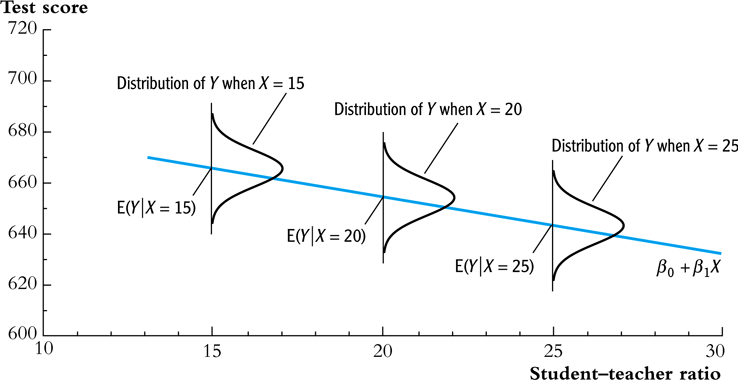
\includegraphics[width=\textwidth]{./figure/fig-4-4}
        \caption{Homoskedasticity}
        \label{fig:homo1}
    \end{subfigure}
    ~ %add desired spacing between images, e. g. ~, \quad, \qquad, \hfill etc. 
      %(or a blank line to force the subfigure onto a new line)
    \begin{subfigure}[!ht]{0.85\textwidth}
        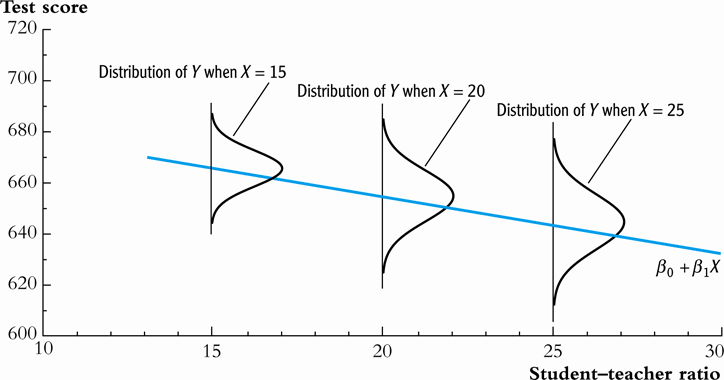
\includegraphics[width=\textwidth]{./figure/fig-5-2}
        \caption{Heteroskedasticity}
        \label{fig:hetero1}
    \end{subfigure}
    \caption{Homoskedasticity Versus Heteroskedasticity}\label{fig:homovshetero}
\end{figure}


\subsection{Mathematical implications of homoskedasticity}
\label{sec:org93c84e8}

\subsubsection*{Unbiasedness, consistency, and the asymptotic distribution}
\label{sec:orge43d4c2}

As long as the least squares assumptions holds, whether the error
term, \(u_i\), is homoskedastic or heteroskedastic does not affect
unbiasedness, consistency, and the asymptotic normal distribution
of the OLS estimators.
\begin{itemize}
\item The unbiasedness requires that \(E(u_i|X_i) = 0\)
\item The consistency requires that \(E(X_i u_i) = 0\), which is true if
\(E(u_i|X_i)=0\).
\item The asymptotic normal distribution requires additionally that
\(\var((X_i-\mu_X)u_i) < \infty\), which still holds as long as
Assumption 3 holds, that is, no extreme outliers of \(X_i\).
\end{itemize}

\subsubsection*{Efficiency}
\label{sec:orgf1fc015}

The existence of heteroskedasticity affects the efficiency of the
OLS estimator
\begin{itemize}
\item Suppose \(\hat{\beta}_1\) and \(\tilde{\beta}_1\) are both unbiased
estimators of \(\beta_1\). Then, \(\hat{\beta}_1\) is said to be more
\textbf{efficient} than \(\tilde{\beta}_1\) if \(\var(\hat{\beta}_1) <
  \var(\tilde{\beta}_1)\).
\item When the errors are homoskedastic, the OLS estimators
\(\hat{\beta}_0\) and \(\hat{\beta}_1\) are efficient among all
estimators that are linear in \(Y_1, \ldots, Y_n\) and are unbiased,
conditional on \(X_1, \ldots, X_n\).

\item See the Gauss-Markov Theorem below.
\end{itemize}


\subsection{The homoskedasticity-only variance formula}
\label{sec:org7fa009d}

Recall that we can write \(\hat{\beta}_1\) as
\begin{equation*}
\hat{\beta}_1 = \beta_1 + \frac{\sum_i (X_i - \bar{X})u_i}{\sum_i
(X_i - \bar{X})^2} 
\end{equation*} 

Therefore, if \(u_i\) for \(i=1, \ldots, n\) is
homoskedastic and \(\sigma^2\) is known, then
\begin{equation}
\label{eq:vbeta-1a} \var(\hat{\beta}_1 | X_i) = \frac{\sum_i (X_i -
\bar{X})^2 \var(u_i|X_i)}{\left[\sum_i (X_i - \bar{X})^2\right]^2} =
\frac{\sigma^2}{\sum_i (X_i - \bar{X})^2} 
\end{equation} 

When \(\sigma^2\) is unknown, then we use \(s^2_u = 1/(n-2) \sum_i
\hat{u}_i^2\) as an estimator of \(\sigma^2\). Thus, the
homoskedasticity-only estimator of the variance of \(\hat{\beta}_1\) is
\begin{equation}
\label{eq:vbeta-1b} \tilde{\sigma}^2_{\hat{\beta}_1} =
\frac{s^2_u}{\sum_i (X_i - \bar{X})^2} 
\end{equation} 

And the homoskedasticity-only standard error is \(SE(\hat{\beta}_1) =
\sqrt{\tilde{\sigma}^2_{\hat{\beta}_1}}\).

Recall that the heteroskedasticity-robust standard error is
\begin{equation*}
SE(\hat{\beta}_1) = \sqrt{\hat{\sigma}^2_{\hat{\beta}_1}}
\end{equation*} 
where
\begin{equation*}
\hat{\sigma}^2_{\hat{\beta}_1} = \frac{1}{n} \frac{\frac{1}{n-2}
\sum_{i=1}^n (X_i - \bar{X})^2 \hat{u}^2_i}{\left[ \frac{1}{n}
\sum_{i=1}^n (X_i - \bar{X})^2 \right]^2} 
\end{equation*} 
which is also referred to as Eicker-Huber-White standard errors.


\subsection{What does this mean in practice?}
\label{sec:org72a5d02}

\begin{itemize}
\item Heteroskedasticity is common in cross-sectional data. If you do not
have strong beliefs in homoskedasticity, then it is always safer to
report the heteroskedasticity-robust standard errors and use these
to compute the robust t-statistic.
\item In most software, the default setting is to report the
homoskedasticity-only standard errors. Therefore, you need to
manually add the option for the robust estimation. 

\begin{itemize}
\item In R, you can use the following codes
\begin{verbatim}
library(lmtest)
model1 <- lm(testscr ~ str, data = classdata)
coeftest(model1, vcov = vcovHC(model1, type="HC1"))
\end{verbatim}

\item In STATA, you can use
\begin{verbatim}
regress testscr str, robust
\end{verbatim}
\end{itemize}
\end{itemize}


\section{The Theoretical Foundations of Ordinary Least Squares}
\label{sec:org30925e8}
\subsection{The Gauss-Markov conditions}
\label{sec:orgb4f28ba}
We have already known the least squares assumptions: for \(i = 1,
\ldots, n\), (1) \(E(u_i|X_i) =
0\), (2) \((X_i, Y_i)\) are i.i.d., and (3) large outliers are unlikely. 

The Gauss-Markov conditions provide anther version of these
assumptions plus the assumption of homoskedastic errors. 

\subsubsection*{The Gauss-Markov conditions}
\label{sec:org4a00d01}
For \(\mathbf{X} = [X_1, \ldots, X_n]\) \footnote{Here I use the vector
notation to represent all observations of \(X_i\) for \(i=1, \ldots,
n\). We will formally introduce the matrix notation for a linear
regression model and the OLS estimation in the next lecture.}
\begin{enumerate}
\item \(E(u_i| \mathbf{X}) = 0\)
\item \(\var(u_i | \mathbf{X}) = \sigma^2_u,\, 0 < \sigma^2_u < \infty\)
\item \(E(u_i u_j | \mathbf{X}) = 0,\, i \neq j\)
\end{enumerate}

\subsubsection*{From the three Least Squares Assumptions and the homoskedasticity assumption to the Gauss-Markov conditions}
\label{sec:org9bcb6e8}
Note that the conditional expectations in the G-M conditions are in
terms of all observations \(\mathbf{X}\), not just one observation,
\(X_i\). However, all the G-M conditions can be derived from the least
squares assumptions plus the homoskedasticity assumption. Specifically,

\begin{itemize}
\item Assumptions (1) and (2) imply \(E(u_i | \mathbf{X}) = E(u_i | X_i) =
  0\).
\item Assumptions (1) and (2) imply \(\var(u_i| \mathbf{X}) =
  \var(u_i | X_i)\). With the homoskedasticity assumption, \(\var(u_i |
  X_i) = \sigma^2_u\), Assumption (3) then implies \(0 < \sigma^2_u < \infty\).
\item Assumptions (1) and (2) imply that \(E(u_i u_j | \mathbf{X}) = E(u_i
  u_j | X_i, X_j) = E(u_i|X_i) E(u_j|X_j) = 0\).
\end{itemize}

\subsection{Linear conditionally unbiased estimator}
\label{sec:org186b0ff}
\subsubsection*{The general form of a linear conditionally unbiased estimator of \(\beta_1\)}
\label{sec:orgbf571b9}

The class of linear conditionally unbiased estimators consists of all
estimators of \(\beta_1\) that are linear function of \(Y_i, \ldots, Y_n\)
and that are unbiased, conditioned on \(X_1, \ldots, X_n\). 

For any linear estimator \(\tilde{\beta}_1\), it can be written as
\begin{equation}
\label{eq:beta1-tilde}
\tilde{\beta}_1 = \sum_{i=1}^n a_i Y_i\
\end{equation}
where the weights \(a_i\) for \(i = 1, \ldots, n\) depend on \(X_1, \ldots,
X_n\) but not on \(Y_1, \ldots, Y_n\). 

\(\tilde{\beta}_1\) is conditionally unbiased means that
\begin{equation}
\label{eq:e-beta1-tilde}
E(\tilde{\beta}_1 | \mathbf{X}) = \beta_1\
\end{equation}

By the Gauss-Markov conditions, from Equation (\ref{eq:beta1-tilde}),  we can have
\begin{equation*}
\begin{split}
E(\tilde{\beta}_1 | \mathbf{X}) &= \sum_i a_i E(\beta_0 + \beta_1 X_i + u_i | \mathbf{X}) \\
&= \beta_0 \sum_i a_i + \beta_1 \sum_i a_i X_i
\end{split}
\end{equation*}

For Equation (\ref{eq:e-beta1-tilde}) being satisfied with any
\(\beta_0\) and \(\beta_1\), we must have
\[ \sum_i a_i = 0 \text{ and } \sum_i a_iX_i = 1 \]

\subsubsection*{The OLS esimator \(\hat{\beta}_1\) is a linear conditionally unbiased estimator}
\label{sec:org7311d3e}

We have known that \(\hat{\beta}_1\) is unbiased both conditionally and
unconditionally. Next, we show that it is linear. 
\[ \hat{\beta}_1 = \frac{\sum_i (X_i - \bar{X})(Y_i - \bar{Y})}{\sum_i
(X_i - \bar{X})^2} = \frac{\sum_i (X_i - \bar{X})Y_i}{\sum_i
(X_i - \bar{X})^2} = \sum_i \hat{a}_i Y_i \]
where the weights are
\[ \hat{a}_i = \frac{X_i - \bar{X}}{\sum_i (X_i - \bar{X})^2}, \text{
for } i = 1, \ldots, n \] 
Since \(\hat{\beta}_1\) is a linear conditionally unbiased estimator, we
must have
\[ \sum_i \hat{a}_i = 0 \text{ and } \sum_i \hat{a}_i X_i = 1  \]
which can be simply verified.

\subsection{The Gauss-Markov Theorem}
\label{sec:org430ff29}
The Gauss-Markov Theorem for \(\hat{\beta}_1\) states
\phantomsection
\label{org2c15ec0}
\begin{quote}
If the Gauss-Markov conditions hold, then the OLS estimator
\(\hat{\beta}_1\) is the *B*est (most efficient) *L*inear conditionally
*U*nbiased *E*stimator (BLUE).
\end{quote}

The theorem can also be applied to \(\hat{\beta}_0\).

The proof of the Gauss-Markov theorem is in Appendix 5.2. A key in
this proof is that we can rewrite the expression of any linear
conditionally unbiased estimator \(\tilde{\beta}_1\) as
\[ \tilde{\beta}_1 = \sum_i a_i Y_i = \sum_i (\hat{a}_i + d_i)Y_i =
\hat{\beta}_1 + \sum_i d_i Y_i \]
And the goal of
the proof is to show that
\[ \var(\hat{\beta}_1 | \mathbf{X}) \leq \var(\tilde{\beta}_1 |
\mathbf{X}) \]
The equality holds only when \(\tilde{\beta}_1 = \hat{\beta}_1\). 

\subsection{The limitations of the Gauss-Markov theorem}
\label{sec:org520d753}
\begin{enumerate}
\item The Gauss-Markov conditions may hold in practice. Any violation of
the Gauss-Markov conditions will result in the OLS estimator not
being BLUE. The table below summarizes the cases in which a kind of
violation occurs, the consequences of such violation to the OLS
estimators, and possible remedies.

\begin{table}[htbp]
\caption{Summary of Violations of the Gauss-Markov Theorem}
\centering
\small
\begin{tabular}{p{4cm}|p{5.5cm}|p{2.5cm}|p{3.4cm}}
\toprule
Violation & Cases & Consequences & Remedies\\
\midrule
\(E(u \mid X) \neq 0\) & omitted variables, endogeneity & biased & more \$X\$'s, IV method\\
\(\var(u_i\mid X)\) not constant & heteroskedasticity & inefficient & WLS, GLS, HCCME\\
\(E(u_{i}u_{j}\mid X) \neq 0\) & autocorrelation & inefficient & GLS, HAC\\
\bottomrule
\end{tabular}
\end{table}

\item There are other candidate estimators that are not linear and
conditionally unbiased; under some conditions, these estimators are
more efficient than the OLS estimators.
\end{enumerate}

\section{Using the t-Statistic in Regression When the Sample Size is Small}
\label{sec:org0b6b9b7}
\subsection{The classical assumptions of the least squares estimation}
\label{sec:org923f997}
We first expand the OLS assumptions by two additional ones. One is the
assumption of the homoskedastic errors, and another one is the
assumption that the conditional distribution of \(u_i\) given \(X_i\) is
the normal distribution, i.e., \(u_i \sim N(0,
\sigma^2_u) \text{ for } i = 1, \ldots, n\). 

All these assumptions together are often referred to as the classical
assumptions of the least squares estimation. 
For \(i = 1, 2, \ldots, n\)
\begin{itemize}
\item Assumption 1: \(E(u_i | X_i) = 0\) (exogeneity of \(X\))
\item Assumption 2: \((X_i, Y_i)\) are i.i.d. (IID of \(X, Y, \text{ and }
                   u\))
\item Assumption 3: \(0 < E(X_i^4) < \infty\) and \(0 < E(Y_i^4) < \infty\)
(No large outliers)
\item Extended Assumption 4: \(\var(u_i | X_i) = \sigma^2_u, \text{ and } 0 <
                   \sigma^2_u < \infty\) (homoskedasticity)
\item Extended Assumption 5: \(u_i | X_i \sim N(0, \sigma^2_u)\) (normality)
\end{itemize}

\subsection{The t-Statistic and the Student-t Distribution}
\label{sec:org69b372d}
Under all the classical assumptions, we can construct the
t-statistic for hypothesis testing of a single coefficient. Even with
a small samples, the t-statistic has an exact Student-t distribution. 

\subsubsection*{The t-statistic is for \(\beta_1\)}
\label{sec:org503fd5d}

\[H_0: \beta_1 = \beta_{1,0} \text{ vs } H_1: \beta_1 \neq \beta_{1,0}\]
\begin{equation}
t = \frac{\hat{\beta}_1 - \beta_{1,0}}{\hat{\sigma}_{\hat{\beta}_1}}
\end{equation}
where
\begin{equation*}
\hat{\sigma}^2_{\hat{\beta}_1} = \frac{s^2_u}{\sum_i (X_i - \bar{X})^2} \text{ and } s^2_u = \frac{1}{n-2}\sum_i \hat{u}_i^2
\end{equation*}
the former of which is the homoskedasticity-only standard error of
\(\hat{\beta}_1\) and the latter is the standard error of the
regression. 

\subsubsection*{The Student-t distribution of \(t\)}
\label{sec:org86d2817}

The t statistic can be rewritten as
\begin{equation}
\label{eq:t-stat-b1a}
t = \frac{(\hat{\beta}_1 - \beta_{1,0})/\sigma_{\hat{\beta}_1}}{\sqrt{\frac{\hat{\sigma}^2_{\hat{\beta}_1}}{\sigma^2_{\hat{\beta}_1}}}} 
= \frac{z_{\hat{\beta}_1}}{\sqrt{\frac{s^2_u}{\sigma^2_u}}} = \frac{z_{\hat{\beta}_1}}{\sqrt{\frac{W}{n-2}}}
\end{equation}
where 

\[\sigma^2_{\hat{\beta}_1} = \frac{\sigma^2_u}{\sum_i (X_i -
\bar{X})^2} \] 

is the homoskedasticity-only variance of
\(\hat{\beta}_1\) when the variance of errors \(\sigma^2_u\) is known.  

\[
z_{\hat{\beta}_1} =\frac{\hat{\beta}_1 -
\beta_{1,0}}{\sigma_{\hat{\beta}_1}} 
\] 

is the z-statistic which has a standard normal distribution, that is,
\(z_{\hat{\beta}_1} \sim N(0, 1)\)

\[ 
W = (n-2)\frac{s^2_u}{\sigma^2_u} =
\frac{\sum_i\hat{u}_i^2}{\sigma^2_u} = \sum_i
\left(\frac{\hat{u}_i}{\sigma_u}\right)^2
 \] 

It can be shown that W is the sum of squares of \((n-2)\) independent
standard normally distributed variables, which results in a
chi-squared distribution with \((n-2)\) degrees of freedom. That is, \(W
\sim \chi^2(n-2)\), which is also independent of
\(z_{\hat{\beta}_1}\). Therefore, the t-statistic in Equation
(\ref{eq:t-stat-b1a}), as the ratio of \(z_{\hat{\beta}_1}\) and
\(\sqrt{W/(n-2)}\), is distributed as \(t(n-2)\).
\end{document}